\documentclass{article}
\usepackage{tikz}
\usetikzlibrary{patterns}
\usepackage{subcaption}
\usepackage[margin=0.5in]{geometry}

\begin{document}

\begin{figure}[ht]
    \centering
    \begin{subfigure}{0.2375\textwidth}
        \centering
        \resizebox{\textwidth}{!}{\input{dual_projection_graphs_a.tex}}
        \caption{Full Dual Graph $G^*$}
    \end{subfigure}
    \hfill
    \begin{subfigure}{0.2375\textwidth}
        \centering
        \resizebox{\textwidth}{!}{\input{dual_projection_graphs_b.tex}}
        \caption{Red-Green Projection}
    \end{subfigure}
    \hfill
    \begin{subfigure}{0.2375\textwidth}
        \centering
        \resizebox{\textwidth}{!}{        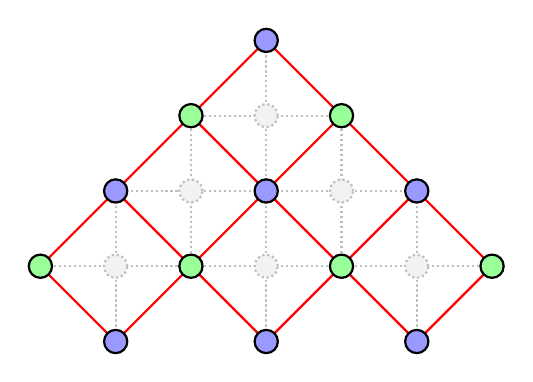
\begin{tikzpicture}[scale=0.7]
            \draw[gray!50, densely dotted, thick] (2.7314, 1.3657) -- (4.0971, 1.3657);
            \draw[gray!50, densely dotted, thick] (1.3657, 2.7314) -- (1.3657, 1.3657);
            \draw[gray!50, densely dotted, thick] (-1.3657, 2.7314) -- (-1.3657, 4.0971);
            \draw[gray!50, densely dotted, thick] (0, 1.3657) -- (-1.3657, 1.3657);
            \draw[gray!50, densely dotted, thick] (0, 4.0971) -- (-1.3657, 4.0971);
            \draw[gray!50, densely dotted, thick] (2.7314, 1.3657) -- (1.3657, 1.3657);
            \draw[gray!50, densely dotted, thick] (0, 1.3657) -- (1.3657, 1.3657);
            \draw[gray!50, densely dotted, thick] (-1.3657, 2.7314) -- (-1.3657, 1.3657);
            \draw[gray!50, densely dotted, thick] (-2.7314, 1.3657) -- (-1.3657, 1.3657);
            \draw[gray!50, densely dotted, thick] (0, 4.0971) -- (1.3657, 4.0971);
            \draw[gray!50, densely dotted, thick] (-2.7314, 1.3657) -- (-4.0971, 1.3657);
            \draw[gray!50, densely dotted, thick] (1.3657, 2.7314) -- (1.3657, 4.0971);
            \draw[gray!50, densely dotted, thick] (0, 2.7314) -- (-1.3657, 2.7314);
            \draw[gray!50, densely dotted, thick] (-2.7314, 2.7314) -- (-1.3657, 2.7314);
            \draw[gray!50, densely dotted, thick] (0, 2.7314) -- (0, 1.3657);
            \draw[gray!50, densely dotted, thick] (0, 2.7314) -- (0, 4.0971);
            \draw[gray!50, densely dotted, thick] (-2.7314, 2.7314) -- (-2.7314, 1.3657);
            \draw[gray!50, densely dotted, thick] (0, 5.4628) -- (0, 4.0971);
            \draw[gray!50, densely dotted, thick] (2.7314, 2.7314) -- (1.3657, 2.7314);
            \draw[gray!50, densely dotted, thick] (-2.7314, 0) -- (-2.7314, 1.3657);
            \draw[gray!50, densely dotted, thick] (0, 2.7314) -- (1.3657, 2.7314);
            \draw[gray!50, densely dotted, thick] (0, 0) -- (0, 1.3657);
            \draw[gray!50, densely dotted, thick] (2.7314, 2.7314) -- (2.7314, 1.3657);
            \draw[gray!50, densely dotted, thick] (2.7314, 0) -- (2.7314, 1.3657);
            \draw[red, thick] (-1.3657, 4.0971) -- (0, 5.4628);
            \draw[red, thick] (1.3657, 4.0971) -- (0, 2.7314);
            \draw[red, thick] (4.0971, 1.3657) -- (2.7314, 2.7314);
            \draw[red, thick] (-1.3657, 4.0971) -- (0, 2.7314);
            \draw[red, thick] (1.3657, 1.3657) -- (2.7314, 0);
            \draw[red, thick] (-1.3657, 1.3657) -- (-2.7314, 0);
            \draw[red, thick] (1.3657, 4.0971) -- (2.7314, 2.7314);
            \draw[red, thick] (-1.3657, 1.3657) -- (0, 0);
            \draw[red, thick] (1.3657, 1.3657) -- (0, 0);
            \draw[red, thick] (4.0971, 1.3657) -- (2.7314, 0);
            \draw[red, thick] (1.3657, 1.3657) -- (0, 2.7314);
            \draw[red, thick] (-4.0971, 1.3657) -- (-2.7314, 2.7314);
            \draw[red, thick] (-1.3657, 1.3657) -- (0, 2.7314);
            \draw[red, thick] (1.3657, 4.0971) -- (0, 5.4628);
            \draw[red, thick] (-1.3657, 1.3657) -- (-2.7314, 2.7314);
            \draw[red, thick] (1.3657, 1.3657) -- (2.7314, 2.7314);
            \draw[red, thick] (-4.0971, 1.3657) -- (-2.7314, 0);
            \draw[red, thick] (-1.3657, 4.0971) -- (-2.7314, 2.7314);
            \filldraw[fill=blue!40, draw=black, thick] (-2.7314, 0) circle (6pt);
            \filldraw[fill=blue!40, draw=black, thick] (0, 0) circle (6pt);
            \filldraw[fill=blue!40, draw=black, thick] (2.7314, 0) circle (6pt);
            \filldraw[fill=blue!40, draw=black, thick] (-2.7314, 2.7314) circle (6pt);
            \filldraw[fill=blue!40, draw=black, thick] (0, 2.7314) circle (6pt);
            \filldraw[fill=blue!40, draw=black, thick] (2.7314, 2.7314) circle (6pt);
            \filldraw[fill=blue!40, draw=black, thick] (0, 5.4628) circle (6pt);
            \filldraw[fill=gray!10, draw=gray!50, densely dotted, thick] (-2.7314, 1.3657) circle (6pt);
            \filldraw[fill=gray!10, draw=gray!50, densely dotted, thick] (0, 1.3657) circle (6pt);
            \filldraw[fill=gray!10, draw=gray!50, densely dotted, thick] (2.7314, 1.3657) circle (6pt);
            \filldraw[fill=gray!10, draw=gray!50, densely dotted, thick] (-1.3657, 2.7314) circle (6pt);
            \filldraw[fill=gray!10, draw=gray!50, densely dotted, thick] (1.3657, 2.7314) circle (6pt);
            \filldraw[fill=gray!10, draw=gray!50, densely dotted, thick] (0, 4.0971) circle (6pt);
            \filldraw[fill=green!40, draw=black, thick] (-4.0971, 1.3657) circle (6pt);
            \filldraw[fill=green!40, draw=black, thick] (-1.3657, 1.3657) circle (6pt);
            \filldraw[fill=green!40, draw=black, thick] (1.3657, 1.3657) circle (6pt);
            \filldraw[fill=green!40, draw=black, thick] (4.0971, 1.3657) circle (6pt);
            \filldraw[fill=green!40, draw=black, thick] (-1.3657, 4.0971) circle (6pt);
            \filldraw[fill=green!40, draw=black, thick] (1.3657, 4.0971) circle (6pt);
        \end{tikzpicture}
}
        \caption{Green-Blue Projection}
    \end{subfigure}
    \vspace{0.5cm}
    \begin{subfigure}{0.2375\textwidth}
        \centering
        \resizebox{\textwidth}{!}{\input{dual_projection_graphs_d.tex}}
        \caption{Blue-Red Projection}
    \end{subfigure}
    
    \vspace{0.5cm}
    \caption{Full Dual Graph $G^*$}
\end{figure}

\end{document}